\section{Shunt-Widerstand}

Der Shunt-Widerstand ist ein Widerstand, welche parallel zum Josephson Kontakt in die Schaltung eingebaut ist. Um diesen zu bestimmen $R_\mathrm{S}$ wird die bei $T = \SI{4.2}{\kelvin}$ und $B = \SI{0}{\tesla}$ aufgenommeneStrom-Spannungs-Kennlinie analysiert. In Abbildung \ref{fig:IVShunt} ist die gemessene Kennlinie zu sehen. Es wird überhalb und unterhalb des Sprungs bei $U = 2\Delta / e$ eine Gerade angelegt. Somit lässt sich der Gesamt- und Shunt-Widerstand bestimmen. Da $U$ über $I$ aufgetragen wird, ergibt sich aus den Steigungen der Geraden direkt der Widerstand im jeweiligen Bereich.Die Werte sind in Tabelle \ref{tab:Shunt} zusammengefasst.

\begin{figure}
    \centering
    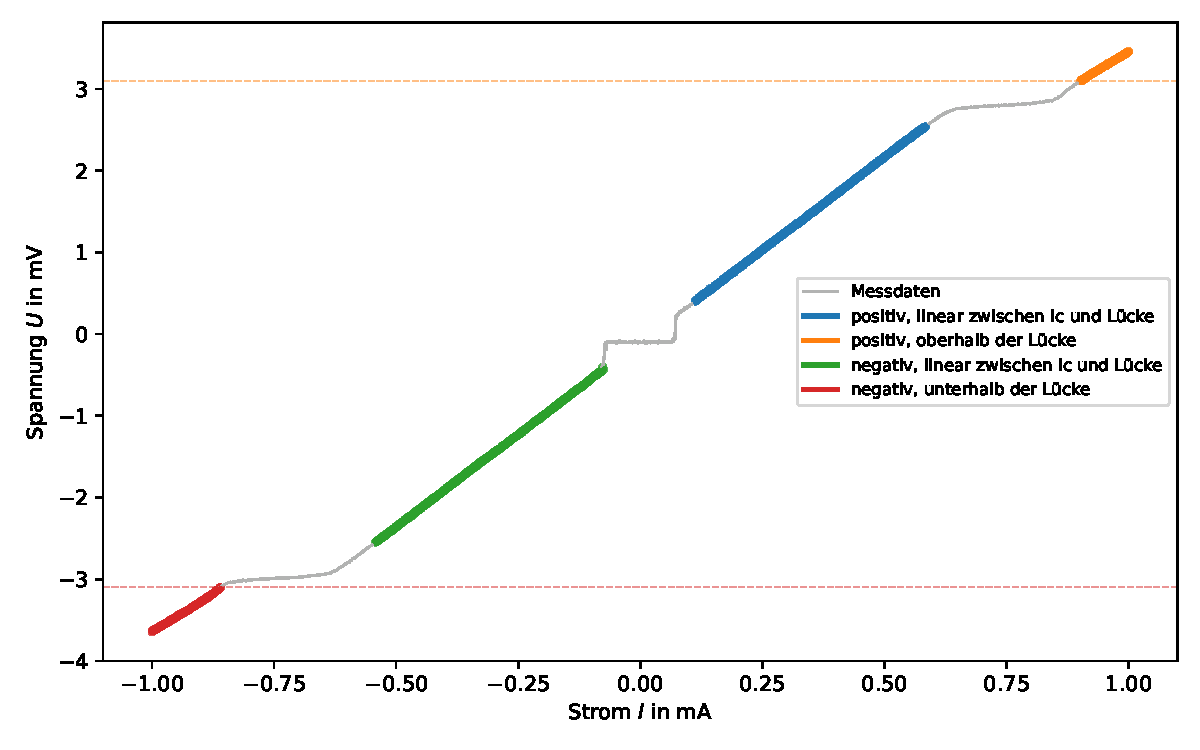
\includegraphics[width=0.8\textwidth]{Leonard/Plots/Shunt_fits_4p191K.pdf}
    \caption{Strom-Spannungs-Kennlinie bei $T = \SI{4.2}{\kelvin}$ und $B = \SI{0}{\tesla}$. Die eingefärbten Bereiche zeigen jeweils die Bereiche an in denen gefittet wurde.}
    \label{fig:IVShunt}
\end{figure}

\begin{table}[h]
    \centering
    \caption{Gefittete Werte des Gesamt- und Shunt-Widerstandes.}
    \label{tab:Shunt}
    \begin{tabular}{c|c c}
         & Gesamtwiderstand $R_\mathrm{ges}$ & Shunt-Widerstand $R_\mathrm{S}$ \\\hline
        Positiver Bereich & $\SI{4.538+-0.002}{\ohm}$ & $\SI{3.61+-0.01}{\ohm}$ \\
        Negativer Bereich & $\SI{4.529+-0.002}{\ohm}$ & $\SI{3.74+-0.01}{\ohm}$ \\
    \end{tabular}
\end{table}

Werden diese Werte gemittelt, ergibt sich für den Gesamtwiderstand $R_\mathrm{ges} = \SI{4.53+-0.02}{\ohm}$ und für den Shunt-Widerstand $R_\mathrm{S} = \SI{3.68+-0.01}{\ohm}$.

Der Normalleitwiderstand $R_\mathrm{N}$ des Tunnelkontakts lässt sich über
\begin{align}
    \frac{1}{R_\mathrm{ges}} &= \frac{1}{R_\mathrm{N}} + \frac{1}{R_\mathrm{S}}\\
    \Rightarrow R_\mathrm{N} &= \frac{R_\mathrm{S} R_\mathrm{ges}}{R_\mathrm{S} - R_\mathrm{ges}}
\end{align}
bestimmen. Somit ergibt sich $R_\mathrm{N} = \SI{19.6}{\ohm}$.

Mit einer fehlerfortpflanzung ergibt sich ein Fehler von
\begin{equation}
    \Delta R_\mathrm{N} = \frac{1}{\left( \frac{1}{R_{\mathrm{ges}} - \frac{1}{R_{\mathrm{S}}}} \right)^2 } \cdot \frac{\Delta R_{\mathrm{ges}}}{R_{\mathrm{ges}}^2} + \frac{1}{\left( \frac{1}{R_{\mathrm{ges}} - \frac{1}{R_{\mathrm{S}}}} \right)^2 } \cdot \frac{\Delta R_{\mathrm{S}}}{R_{\mathrm{S}}^2} = \SI{0.7}{\ohm}\:.
\end{equation}

Der Stewart-McCumber-Parameter $\beta_\mathrm{C}$ lässt sich mit der gegebenen Kapazität $C=\SI{200}{\femto\farad}$ als
\begin{equation}
    \beta_\mathrm{C} = \frac{2 e I_\mathrm{C} R_\mathrm{ges}^2 C}{\hbar} = 0.748 
\end{equation}
bestimmen. 
Mit einem Fehler von
\begin{equation}
    \Delta \beta_\mathrm{C} = \frac{2 e I_\mathrm{C} C}{\hbar} \cdot 2 R_\mathrm{ges} \cdot \Delta R_\mathrm{ges} = 0.007
\end{equation}
Es gilt also $\beta_\mathrm{C} < 1$ und somit ist der Josephson-Kontakt überdämpft und es liegt eine hysteresefrei Kurve vor.